% !TeX program = lualatex
% !TeX root = menua5.tex
% !TeX spellcheck = de_DE
%\documentclass[a4paper,10pt,notumble]{leaflet}
\documentclass[12pt,a5paper,oneside]{scrreprt}

\usepackage[scaled]{helvet}
\renewcommand\familydefault{\sfdefault} 
\usepackage{fontspec}% for lualatex
\usepackage{polyglossia}
\setdefaultlanguage[]{german}
\setotherlanguage[]{german}
%\usepackage{setspace}
\usepackage{hyperref}
\usepackage{siunitx}
\sisetup{locale = DE}
\DeclareSIUnit[number-unit-product = { } ]
	\EUR{EUR}

\usepackage{graphicx}

\usepackage{titlesec}

\newcommand{\largemenuonly}[1]{#1}
\newcommand{\smallmenuonly}[1]{}

%\usepackage{pgfpages}
%\pgfpagesuselayout{2 on 1}[a4paper,landscape,border shrink=5mm]

\newcommand{\meal}[4]{\textbf{#1}\hspace{3mm}%
\begin{minipage}[t]{8 cm}
\begin{flushleft}
#2\textsuperscript{#3}
\end{flushleft}
\end{minipage}%
\hfill\SI{#4}{\EUR}\\[2mm]}

\titlespacing*{\section}{0pt}{3mm}{2mm}
%\titlespacing*{<command>}{<left>}{<before-sep>}{<after-sep>}

% Allergen-Verzeichnis
\newcommand{\Getreideprodukte}{a}
\newcommand{\Fisch}{b}
\newcommand{\Krebstiere}{c}
\newcommand{\Schwefel}{d} 
\newcommand{\Sellerie}{e} 
\newcommand{\Laktose}{f} 
\newcommand{\Sesamsamen}{g} 
\newcommand{\Nuss}{h} 
\newcommand{\Eier}{i} 
\newcommand{\Lupinen}{j} 
\newcommand{\Senf}{k} 
\newcommand{\Soja}{l} 
\newcommand{\Weichtiere}{m} 
\newcommand{\Erdnuss}{n} 




\begin{document} 
\hypersetup{
  pdftitle={Speisekarte Yen Yen},  
  pdfsubject={Speisekarte},
  pdfauthor={Jonas Stein}
  pdfnewwindow=true
}

\begin{center}
\includegraphics[width=\textwidth]{gfx/yenyen_head_bw_text.png}
\end{center}

% {\Huge Yen Yen Asia Express}\\
{\small Stand vom \today}\\[5mm]
Unser Restaurant hat an Sonn- und Feiertagen geschlossen. Reservierungen und Vorbestellungen für Selbstabholer unter
\begin{center}
{\Huge 02241 / 126 87 72}\\[4mm]

\textbf{Wir kochen ohne Glutamat.}
\end{center}

\section*{Partyservice}
Sie möchten Ihre Gäste in Ihrer Location mit gesunden, \mbox{asiatischen} Speisen verwöhnen?\\ 
Sprechen Sie uns an, wir beraten Sie gern.
\newpage
% !TeX program = lualatex
% !TeX root = menu.tex
% !TeX spellcheck = de_DE
\section*{Erste Stärkung}
diese Gerichte sind \textbf{schnell} zubereitet und sowohl als
\textbf{Vorspeise} als auch als \textbf{Hauptgericht} sehr beliebt
\begin{flushleft}
\meal{X1}{6 Mini-Frühlingsrollen, süßsauer}{\Getreideprodukte, \Soja}{2.00}
\meal{X2}{Pekingsuppe}{\Eier, \Getreideprodukte}{2.20}
%\meal{X3}{Gebratener Reis mit Gemüse und Hühnerfleisch}{\Soja, \Eier, \Getreideprodukte}{4.90}
%\meal{X4}{Gebratene Nudeln mit Gemüse und Hühnerfleisch}{\Soja, \Eier, \Getreideprodukte}{4.90}
\meal{X5}{Krabbenchips}{\Getreideprodukte, \Fisch, \Krebstiere}{1.70}
\meal{X6}{Süßkartoffelchips}{\Getreideprodukte}{1.90}
\meal{X7}{Gebackene Wantan, süßsauer}{\Eier, \Soja,\Getreideprodukte,\Sellerie}{3.50}
\meal{X8}{Gebackener Brokkoli}{\Soja,\Getreideprodukte,\Sellerie,\Eier}{3.50}
\end{flushleft}

\section*{Vorspeisen}
\meal{U1}{Zwei vietnamesische Frühlingsrollen, hausgemacht, süßsauer}{\Getreideprodukte, \Soja, \Eier, \Sellerie}{3.80}
\meal{U2}{Zwei vietnamesische Frühlingsrollen, hausgemacht, pikant}{\Getreideprodukte, \Soja, \Eier, \Sellerie}{3.80}
\meal{U3}{Eine chinesische Frühlingsrolle, hausgemacht, süßsauer}{\Getreideprodukte, \Soja, \Eier, \Sellerie}{3.60}
\meal{U4}{Eine chinesische Frühlingsrolle, hausgemacht, pikant}{\Getreideprodukte, \Soja, \Eier, \Sellerie}{3.60}
\largemenuonly{\newpage}
\section*{Suppen}
\meal{Z1}{Pekingsuppe mit Hühnerfleisch}{\Soja,\Getreideprodukte,\Sellerie,\Eier}{2.20}
\meal{Z2}{Wantansuppe}{\Soja,\Getreideprodukte,\Eier}{3.50}
\meal{Z3}{Gemüsesuppe mit Hühnerfleisch}{\Soja}{3.50}
\meal{Z4}{Gemüsesuppe mit Glasnudeln}{\Soja,\Getreideprodukte}{3.90}
\meal{Z5}{Gemüsesuppe mit Tofu}{\Soja,\Getreideprodukte,\Lupinen}{4.10}
\meal{Z6}{Wantan Suppe Thai-Art}{\Getreideprodukte,\Laktose,\Soja,\Eier}{4.10}
\meal{Z7}{Garnelen-Suppe Thai-Art mit Kokosmilch und Hühnerfleisch (Hauptspeise)}{\Fisch,\Krebstiere,\Weichtiere,\Getreideprodukte,\Laktose}{11.80}

\section*{Vegetarische Spezialitäten}
\meal{V1}{Tofu mit Gemüse}{\Getreideprodukte,\Soja}{8.90}
\meal{V2}{Tofu mit Gemüse in Curry-Soße}{\Getreideprodukte,\Laktose,\Soja}{9.90}
\meal{V3}{Gebratenes Gemüse}{\Getreideprodukte,\Soja}{6.90}
\meal{V4}{Gebratener Brokkoli mit Zwiebeln u. Knoblauch}{\Getreideprodukte,\Soja}{7.90}
\meal{V5}{Gebratene Champignons mit Zwiebeln}{\Getreideprodukte,\Soja}{7.90}
\meal{V6}{Verzaubernder Mond, gebr. Brokkoli in Currysoße mit Kokosmilch und Blumenkohl}{\Getreideprodukte, \Laktose}{8.90}
\meal{V7}{Kleiner Salat der Saison}{\Soja}{4.90}
\meal{V8}{Gebr. Gemüse in Curry-Soße}{\Getreideprodukte, \Laktose}{7.90}

\largemenuonly{\newpage}
\section*{Hühnerfleisch}
\meal{H1}{gebraten mit gebratenem Reis}{\Getreideprodukte,\Eier,\Soja}{4.90}
\meal{H2}{gebraten mit gebratenen Nudeln}{\Getreideprodukte,\Eier,\Soja}{4.90}
\meal{H3}{gebraten in Currysoße mit Kokosmilch}{\Laktose, \Getreideprodukte}{8.90}
\meal{H4}{auf Thai Art, scharf, mit Kokosmilch}{\Getreideprodukte, \Soja}{8.90}
\meal{H5}{gebr. mit Bambus und Morcheln}{\Getreideprodukte, \Soja}{7.90}
\meal{H6}{gebraten mit Gemüse der Saison}{\Getreideprodukte, \Soja}{7.90}
\meal{H7}{im Teigmantel gebacken mit Gemüse und Reis, süßsauer}{\Eier, \Getreideprodukte, \Soja, \Sellerie}{7.90}
\meal{H8}{im Teigmantel gebacken mit Gemüse und Reis, pikant}{\Eier, \Getreideprodukte, \Soja}{7.90}
\meal{H9}{gebr. mit Gemüse in süßsaurer Soße}{\Getreideprodukte, \Sellerie}{7.90}
\meal{H10}{gebr. mit Gemüse u. Reis, pikant}{\Getreideprodukte, \Soja}{7.90}
\meal{H11}{Kung Bao-Art, pikant}{\Getreideprodukte, \Nuss, \Soja}{7.90}
\meal{H12}{mit Brokkoli und Knoblauch}{\Getreideprodukte, \Nuss, \Soja}{7.90}
\meal{H13}{mit Ingwer und Zitronengras}{\Getreideprodukte, \Soja}{7.90}
%Thịt nướng xâu
\meal{H14}{als Saté-Spieße süßsauer}{\Getreideprodukte, \Sellerie}{10.90}
\meal{H15}{als Saté-Spieße mit Erdnuss-Soße}{\Getreideprodukte, \Soja, \Erdnuss, \Laktose}{11.90}
\meal{H16}{als Saté-Spieße mit spezial Hoisin-Sauce}{\Getreideprodukte, \Soja, \Sesamsamen, \Laktose}{10.90} %
\meal{H17}{Kindermenü; Chicken Nuggets mit Pommes frites}{\Eier, \Getreideprodukte}{3.90} %

\largemenuonly{\newpage}
\section*{Kross gebratenes Entenbrustfilet}
in einer knusprigen Hülle frisch gebraten serviert\\
\meal{E1}{mit Gemüse und süßsaurer Soße}{\Getreideprodukte, \Sellerie, \Eier, \Soja}{9.90}
\meal{E2}{mit Gemüse und pikanter Soße}{\Getreideprodukte, \Sellerie, \Eier, \Soja}{9.90}
\meal{E3}{mit Gemüse und Erdnuss-Soße}{\Getreideprodukte, \Laktose, \Eier, \Erdnuss}{11.90}
\meal{E4}{mit Gemüse und Thaisoße, scharf}{\Getreideprodukte, \Laktose, \Eier}{11.90}
\meal{E5}{mit Gemüse und pikanter Hoisin Soße und Cashewkernen}{\Getreideprodukte, \Laktose, \Eier, \Nuss}{12.90}
\meal{E6}{pikant, mit Champignons und Zwiebeln}{\Getreideprodukte, \Laktose, \Eier}{12.90}
\meal{E7}{mit Gemüse und Currysoße}{\Getreideprodukte, \Laktose, \Eier}{11.90}
\meal{E8}{mit Gemüse, Ingwer und Zitronengras}{\Getreideprodukte, \Eier}{11.90}
\meal{E9}{mit Gemüse in gemahlenen schwarzen Bohnen, scharf}{\Getreideprodukte, \Soja, \Eier}{11.90}
\begin{flushleft}

%\section*{Yen-Yen Menü}
\largemenuonly{\newpage}
\section*{Geheimnisvolle Küchenmärchen}
\meal{Y1}{Überraschungsgericht}{\Laktose, \Getreideprodukte, \Soja, \Nuss, \Sesamsamen, \Sellerie}{10.90}
\meal{Y2}{Y1 mit Ente}{\Laktose, \Getreideprodukte, \Soja, \Nuss, \Sesamsamen, \Sellerie}{12.90}
\meal{Y3}{Drachenteller: Entenbrustfilet auf gebr. Nudeln mit Gemüse und Cashewkernen (scharf)}{\Getreideprodukte, \Eier, \Laktose, \Soja, \Nuss}{13.80}
Gebratene \textbf{Reisbandnudeln} mit...\\
%\meal{Y4}{Gebr. Reisbandnudeln mit Gemüse}{\Getreideprodukte, \Soja}{11.90}
\meal{Y5}{Rinderfiletstreifen}{\Getreideprodukte, \Soja}{15.90}
\meal{Y6}{Hühnerfleisch}{\Getreideprodukte, \Soja}{13.90}
\meal{Y11}{Garnelen}{\Getreideprodukte,\Soja,\Fisch,\Krebstiere}{16.90}
Gebratene \textbf{Reisfadennudeln} mit...\\
%\meal{Y7}{Gebr. Reisfadennudeln mit Gemüse}{\Getreideprodukte, \Soja}{11.90}
\meal{Y8}{Rinderfiletstreifen}{\Getreideprodukte, \Soja}{15.90}
\meal{Y10}{Garnelen}{\Getreideprodukte,\Soja,\Fisch,\Krebstiere}{16.90}
\meal{Y9}{vietnamesischen Frühlingsrollen und Erdnüssen, dazu hausgemachte Limettensoße}{\Getreideprodukte, \Soja, \Eier, \Erdnuss}{14.90}


\largemenuonly{\newpage}
\section*{Saftiges Schweinefleisch}
\meal{P1}{mit Gemüse und pikanter Soße}{\Getreideprodukte,\Soja}{7.90}
\meal{P2}{mit Zwiebeln und pikanter Soße}{\Getreideprodukte,\Soja}{7.90}
\meal{P3}{gebraten, mit süßsaurer Soße}{\Getreideprodukte,\Sellerie,\Soja}{7.90}
\meal{P4}{in Teigmantel, pikant}{\Getreideprodukte,\Sellerie,\Soja}{7.90}
\meal{P5}{in Teigmantel, süßsauer}{\Getreideprodukte,\Sellerie,\Soja}{7.90}

\section*{Spezialitäten vom Rind}
zarte Rinderfiletstreifen kurz angebraten\\
\meal{R1}{pikant}{\Getreideprodukte, \Soja}{8.90}
\meal{R2}{mit Zwiebeln, Sellerie}{\Getreideprodukte, \Soja, \Sellerie}{8.90}
\meal{R3}{mit pikanter Soße aus gemahlenen schwarzen Bohnen}{\Getreideprodukte, \Soja, \Laktose}{8.90}
\meal{R4}{mit Zitronengras und Ingwer}{\Getreideprodukte, \Soja}{8.90}
\meal{R5}{mit Gemüse}{\Getreideprodukte, \Soja}{8.90}
\meal{R6}{mit Champignons, Zwiebeln}{\Getreideprodukte, \Soja}{8.90}
\meal{R7}{Thai Art mit Kokosmilch, scharf}{\Getreideprodukte, \Laktose}{10.80}
\meal{R8}{Mit Brokkoli, Zwiebeln, Knoblauch}{\Getreideprodukte, \Soja}{8.90}

\largemenuonly{\newpage}
\section*{Spezialitäten aus dem Wasser}
\meal{W1}{Norwegischer Premium Lachs mit Gemüse der Saison}{\Fisch, \Getreideprodukte, \Soja, \Krebstiere}{11.90}
\meal{W2}{Norwegischer Premium Lachs mit Gemüse der Saison in Curry-Soße}{\Fisch, \Getreideprodukte, \Laktose, \Krebstiere}{13.80}
\meal{W3}{Norwegischer Premium Lachs mit Kung Bao-Soße}{\Fisch, \Getreideprodukte, \Laktose, \Nuss, \Soja}{13.80}
\meal{W4}{Garnelen Kung Bao Art, scharf}{\Fisch,\Getreideprodukte,\Soja,\Nuss,\Krebstiere}{10.90}
\meal{W5}{Garnelen im Teigmantel}{\Eier \Fisch, \Getreideprodukte, \Soja, \Laktose, \Krebstiere}{10.90}
\meal{W6}{Garnelen mit Ingwer und Zitronengras}{\Fisch, \Getreideprodukte, \Soja, \Krebstiere}{10.90}
\meal{W7}{Garnelen mit gebratenen Nudeln}{\Fisch, \Getreideprodukte, \Soja, \Krebstiere}{12.90}
\meal{W8}{Garnelen mit Gemüse d. Saison}{\Fisch,\Getreideprodukte,\Soja,\Krebstiere}{10.90}
\meal{W9}{Seelachsfilet im Teigmantel mit süßsaurer Soße}{\Getreideprodukte, \Fisch, \Sellerie, \Eier, \Laktose}{9.80}
\vspace{1mm}
\textbf{Alle Hauptgerichte ohne Nudeln werden automatisch mit Jasmin-Duftreis serviert.}

\section*{Extras} 
\meal{+R}{gebratenen Reis als Beilage extra}{~}{2.00}
\meal{+N}{gebratene Nudeln als Beilage extra}{~}{2.00}
\end{flushleft}
\largemenuonly{\newpage}
\section*{Für Kreative}
Stellen Sie sich Ihr Lieblingsgericht unter anderem aus folgenden Zutaten selbst zusammen:
Reis, gebratene Nudeln, Bambus, Brokkoli, Cashewkerne, Ingwer, Zwiebeln, Knoblauch,
Rindfleisch, Schweinefleisch, gebratene Ente, Hühnerfleisch... Preis auf Anfrage.

\section*{Nachspeisen} 
\meal{N1}{gebackene Banane mit Honig}{\Getreideprodukte, \Eier}{3.50}
%\meal{N2}{Vanilleeis mit Früchten garniert}{\Laktose}{2.90}
\meal{N3}{Vanilleeis mit Banane und Schokoladensoße}{\Eier, \Laktose}{3,90}
%\vspace{0.5cm}
\largemenuonly{\newpage}
\section*{Kalte Getränke}
\meal{G1}{Cola (0,2 L)}{~}{1.80}
\meal{G2}{Cola (0,3 L)}{~}{2.10}
\meal{G3}{Fanta (0,2 L)}{~}{1.80}
\meal{G4}{Fanta (0,3 L)}{~}{2.10}
\meal{G5}{Wasser (0,2 L)}{~}{1.80}
\meal{G6}{Wasser (0,3 L)}{~}{2.10}
\meal{G7}{Bitburger alkoholfrei (0,3 L)}{~}{2.10}
\meal{G8}{Malzbier (0,3 L)}{~}{2.20}
\meal{G9}{Bitter Lemon (0,2 L)}{~}{2.20}
\meal{G10}{Ginger Ale (0,2 L)}{~}{2.20}
\meal{G11}{Lychee-Nektar (0,2 L)}{~}{2.20}
\meal{G12}{Mango-Nektar (0,2 L)}{~}{2.20}
\meal{G13}{Orangensaft (0,2 L)}{~}{2.10}
\meal{G14}{Apfelsaft (0,2 L)}{~}{2.10}
\largemenuonly{\newpage}
\section*{Tee und Kaffee}
\meal{J1}{Kaffee}{~}{2.20}
%\meal{J2}{Cappuchino}{\Laktose}{1.90}
\meal{J3}{Kamillentee}{~}{2.20}
\meal{J4}{Jasmintee}{~}{2.20}
\meal{J5}{Drachenperlen (Jasmin Tee)}{~}{2.60}
\meal{J6}{Schwarzer Tee}{~}{2.20}
\meal{J7}{Blumentee (Kännchen)}{~}{5.50}
\meal{J8}{Grüner Tee}{~}{2.20}
\meal{J9}{Früchtetee}{~}{2.20}
\meal{J10}{Pfefferminztee}{~}{2.20}
\meal{J11}{Espresso}{~}{2.20}

\section*{Alkoholische Getränke}
\meal{Q1}{Gaffel Kölsch 4.8 \% (0,3 L)}{~}{2.10}
\meal{Q2}{Bitburger Pils 4.8 \% (0,3 L)}{~}{2.10}
\meal{Q3}{Paulaner Weizen 5.5 \% (0,5 L)}{~}{3.10}
\meal{Q4}{Pflaumenwein 10 \% (0,04 L)}{~}{2.50}
\meal{Q5}{Rotwein Bréjou Bordeaux\\ 12.5\,\% (0,2\,L)}{~}{4.90}
\meal{Q6}{Weißwein Riesling Kalkstein Qualitätswein Pfalz 12.5 \% (0,2 L)}{~}{4.90}
%\meal{Q7}{Sake (Reiswein) XX \% (0,04 L)}{~}{2.50}


\newpage
\section*{Allergenkennzeichnung}
\begin{verbatim}
nach EU-Lebensmittelinformationsverordnung
a Getreideprodukte (glutenhaltig) 
b Fisch
c Krebstiere
d Schwefeldioxide und Sulfite 
e Sellerie
f Milch und Laktose
g Sesamsamen
h Nüsse
i Eier
j Lupinen
k Senf
l Soja
m Weichtiere
n Erdnüsse
\end{verbatim}
Informationen über Zutaten in unseren Speisen, die Allergien
oder Unverträglichkeiten auslösen können, erhalten Sie auf Nachfrage
auch bei unseren Mitarbeitern.\\ 
\textbf{Gerne passt unser Koch das Rezept auf Ihre Bedürfnisse an.} %
%\newpage
%\section*{Lage in der Troisdorfer Innenstadt}
%\begin{center}
%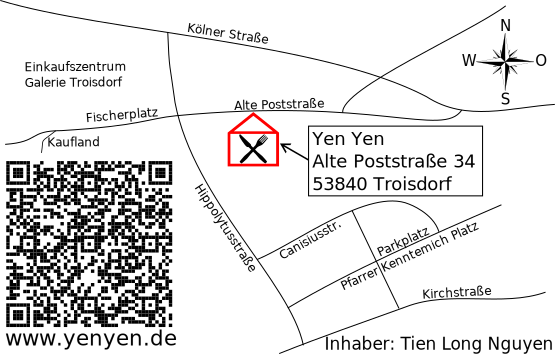
\includegraphics[width=1.0\textwidth]{gfx/map/tdfcity}\\
%\end{center}
%\newpage
%.
%\newpage
%.
\end{document}